
\begin{myex}
	
Sur sa console de jeux, Dorian s'apprête à affronter en duel l'un des trois monstres Thor, Odin et Loki. Ces monstres sont de forces inégales : la probabilité pour que Dorian l'emporte contra Thor; Odin ou Loki est respectivement $\dfrac{1}{4}$, $\dfrac{1}{3}$ et $\dfrac{1}{2}$. De plus Dorian a une chance sur deux d'affronter Thor, et autant de chances de rencontrer Odin que Loki.\\

On considère un duel au hasard et les événements :
\begin{itemize}
	\item $T$ : Dorian combat Thor.
	\item $O$ : Dorian combat Odin.
	\item $L$ : Dorian combat Loki.
	\item $G$ : Dorian gagne son combat.
\end{itemize} 


% Set the overall layout of the tree
\tikzstyle{level 1}=[level distance=3.5cm, sibling distance=3.5cm]
\tikzstyle{level 2}=[level distance=3.5cm, sibling distance=2cm]

% Define styles for bags and leafs
\tikzstyle{bag} = [text width=4em, text centered]
\tikzstyle{end} = [circle, minimum width=3pt,fill, inner sep=0pt]

% The sloped option gives rotated edge labels. Personally
% I find sloped labels a bit difficult to read. Remove the sloped options
% to get horizontal labels. 
\begin{tikzpicture}[grow=right, sloped]
\node[bag] {}
    child {
        node[bag] {L}        
            child {
                node[end, label=right:
                    {$\bar{G} \qquad  \rightarrow p(L \cap \bar{G}) = \dfrac{1}{4} \times \dfrac{1}{2} = \dfrac{1}{8}$}] {}
                edge from parent
                node[below] {$P_L(\bar{G})=\dfrac{1}{2}$}
                %node[below]  {$\frac{4}{9}$}
            }
            child {
                node[end, label=right:
                    {$G \qquad  \rightarrow p(L \cap G) = \dfrac{1}{4} \times \dfrac{1}{2} = \dfrac{1}{8}$}] {}
                edge from parent
                node[above] {{\footnotesize $P_L(G)=\dfrac{1}{2}$}}
                %node[below]  {$\frac{5}{9}$}
            }
            edge from parent 
            %node[above] {$W$}
            node[below]  {$P(L)=\dfrac{1}{4}$}
    }
    child {
        node[bag] {O}        
        child {
                node[end, label=right:
                    {$\bar{G}  \qquad  \rightarrow p(O \cap \bar{G}) = \dfrac{1}{4} \times \dfrac{2}{3} = \dfrac{1}{6}$}] {}
                edge from parent
                %node[above] {$B$}
                node[below]  {{\footnotesize $P_O(\bar{G})=\dfrac{2}{3}$}}
            }
            child {
                node[end, label=right:
                    {$G  \qquad  \rightarrow p(O \cap G) = \dfrac{1}{4} \times \dfrac{1}{3} = \dfrac{1}{12}$}] {}
                edge from parent
                node[above] {{\footnotesize $P_O(G)=\dfrac{1}{3}$}}
%                node[below]  {$\frac{6}{9}$}
            }
        edge from parent         
            %node[above] {$B$}
            node[above]  {$P(O)=\dfrac{1}{4}$}
    }
    child {
    	node[bag] {T}        
    	child {
    		node[end, label=right:
    		{$\bar{G} \qquad  \rightarrow p(T \cap \bar{G}) = \dfrac{1}{2} \times \dfrac{3}{4} = \dfrac{3}{8}$}] {}
    		edge from parent
    		%node[above] {$B$}
    		node[below]  {{\footnotesize $P_T(\bar{G})=\dfrac{3}{4}$}}
    	}
    	child {
    		node[end, label=right:
    		{$G \qquad  \rightarrow p(T \cap G) = \dfrac{1}{2} \times \dfrac{1}{4} = \dfrac{1}{8}$}] {}
    		edge from parent
    		node[above] {$P_T(G)=\dfrac{1}{4}$}
    		%                node[below]  {$\frac{6}{9}$}
    	}
    	edge from parent         
    	%node[above] {$B$}
    	node[above]  {$P(T)=\dfrac{1}{2}$}
    };
\end{tikzpicture}

\vspace*{1cm}
\begin{align*}
p(G) &= p(T \cap G) + p(O \cap G) + p(L \cap G)\\
p(G) &= \dfrac{1}{8} + \dfrac{1}{12} + \dfrac{1}{8}\\
p(G) &= \dfrac{32}{96}\\
p(G) &= \dfrac{1}{3}
\end{align*}

Dorian a une chance sur trois de gagner son duel.
\end{myex}